% 1977 年山西卷第三题：梯形 ABCD（A 左上、D 右上、B 左下、C 右下，上底 AD 短、下底 BC 长），
% M、N 分别为腰 AB、DC 中点，MN 为中位线（实线）；辅助线：DM 延长交 CB 的延长线于 E（虚线 D-M-E），
% E—B 沿底边延长线（虚线）（按源卷第 2 页布局）
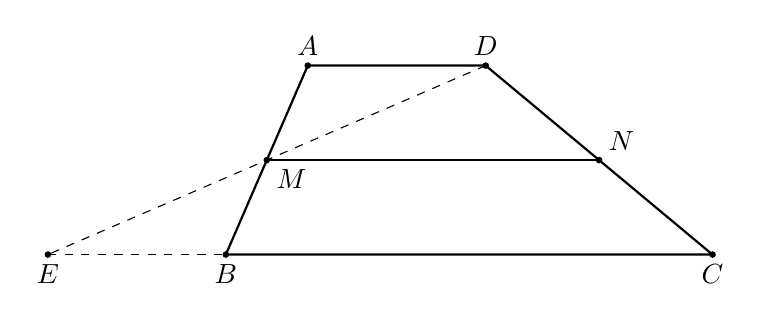
\begin{tikzpicture}[scale=1.0]
  \coordinate (A) at (0,2.4);
  \coordinate (D) at (2.26,2.4);
  \coordinate (B) at (-1.04,0);
  \coordinate (C) at (5.14,0);
  \coordinate (M) at (-0.52,1.2);
  \coordinate (N) at (3.7,1.2);
  \coordinate (E) at (-3.3,0);
  \draw[thick] (A)--(B)--(C)--(D)--cycle;
  \draw[thick] (M)--(N);
  \draw[dashed] (D)--(M)--(E);
  \draw[dashed] (E)--(B);
  \fill (A) circle (1.2pt) node[above] {$A$};
  \fill (D) circle (1.2pt) node[above] {$D$};
  \fill (B) circle (1.2pt) node[below] {$B$};
  \fill (C) circle (1.2pt) node[below] {$C$};
  \fill (M) circle (1.2pt) node[below right] {$M$};
  \fill (N) circle (1.2pt) node[above right] {$N$};
  \fill (E) circle (1.2pt) node[below] {$E$};
\end{tikzpicture}
